\chapter{Fundamentos de las redes neuronales} \label{Capitulo_2}
\begin{itemize}
	\item Supervisado y no supervisado
	\item one-hot encoder
	\item validacion cruzada
	\item dropout, l2
	\item optiizadores
	\item arquitectuas
	\item metricas
\end{itemize}
en la pagina 458 de hands aparece la arquitectura mía


\section{Revisión teórica} \label{Subsec: 3_1}
Puedo introducir los tipos de funciones de activavion. Esta bien explicado en el TFG wuolah o en el articulo de KDD cup 199 de DNN network intrusion.
Puedo añadir overfitting y underfitting.
lo que es aprendizaje supervisado y no supervisao
Partes de una neurona y como trabaja(bias, pesos...)



\section{Introducción}

En la última década, la inteligencia artificial (IA) se ha convertido en un tema popular tanto dentro como fuera de la comunidad científica. Una abundancia de artículos en revistas tecnológicas y no tecnológicas han cubierto los temas de aprendizaje automático (ML, por sus siglas en inglés), aprendizaje profundo (DL, por sus siglas en inglés) e IA. Sin embargo, todavía persiste confusión en torno a IA, ML y DL. Los términos están estrechamente relacionados, pero no son intercambiables. 

En 1956, un grupo de científicos informáticos propuso que las computadoras podrían ser programadas para pensar y razonar, ``que cada aspecto del aprendizaje o cualquier otra característica de la inteligencia podría, en principio, ser descrito tan precisamente que una máquina podría simularlo'' \citep{moor2006dartmouth}. Describieron este principio como ``inteligencia artificial''. En pocas palabras, la IA es un campo enfocado en automatizar tareas intelectuales que normalmente realizan los humanos, y el Machine Learning es un método específico para lograr este objetivo. Es decir, está dentro del ámbito de la IA (Figura \ref{fig:fig1}) \citep{choi2020introduction}. 

\begin{figure}[h!]
    \centering
    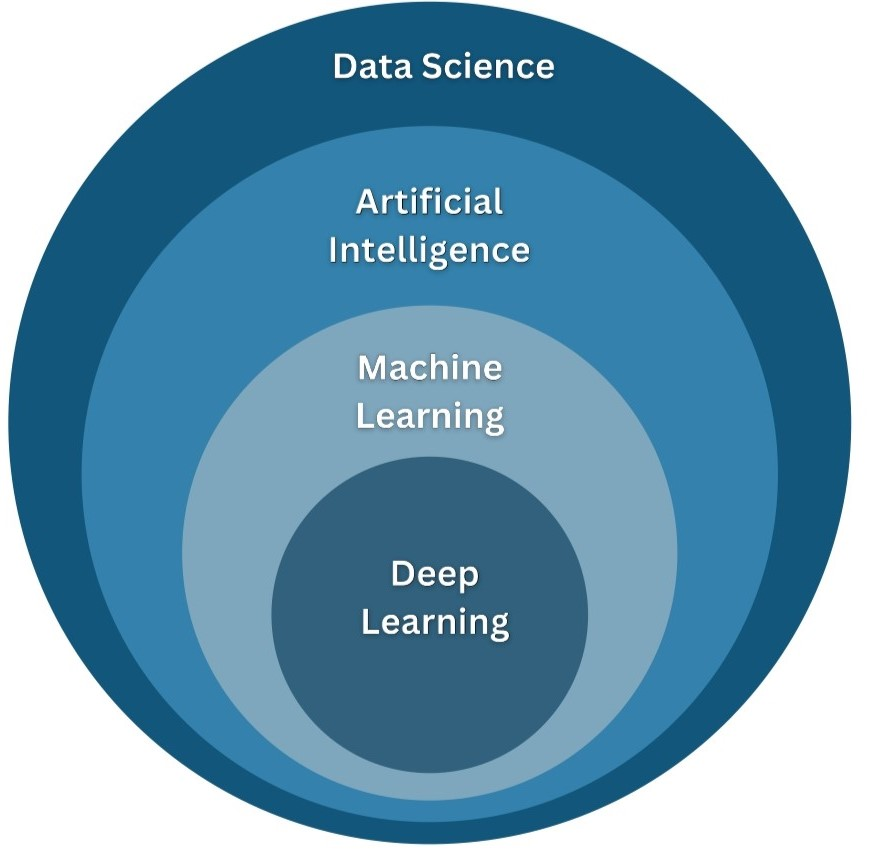
\includegraphics[width=0.4\textwidth]{img/ia.jpg}
    \caption{Relación entre Ciencia de Datos, Inteligencia Artificial, Machine Learning y Deep Learning.}
    \label{fig: ia}
\end{figure}


\section{Aprendizaje Automático}

Por otro lado, el Aprendizaje Automático (ML, por sus siglas en inglés) es la ciencia o el arte de programar ordenadores para que puedan aprender a partir de datos. Arthur Samuel lo definió en 1959 como ``el campo de estudio que otorga a las computadoras la capacidad de aprender sin ser explícitamente programadas''. Más formalmente, según Tom Mitchell (1997), ``se dice que un programa de computadora aprende de la experiencia \(E\) con respecto a alguna tarea \(T\) y alguna medida de rendimiento \(P\), si su rendimiento en \(T\), medido por \(P\), mejora con la experiencia \(E\)'' \citep{geron2022hands}. El aprendizaje automático ha revolucionado numerosos campos, permitiendo a las máquinas realizar tareas que antes requerían intervención humana directa. Desde la conducción autónoma hasta el diagnóstico médico, las aplicaciones del aprendizaje automático son diversas. A diferencia de los métodos tradicionales de programación, donde se codifican reglas explícitas, el aprendizaje automático permite que los sistemas descubran patrones y relaciones directamente a partir de los datos, adaptándose y mejorando con el tiempo.



Un ejemplo de aprendizaje automático es un filtro de spam que, dado ejemplos de correos electrónicos de spam y ejemplos de correos electrónicos normales (no spam, también llamados ``ham''), puede aprender a marcar el spam \citep{geron2022hands}. Los ejemplos que el sistema utiliza para aprender se llaman el conjunto de entrenamiento. Cada ejemplo de entrenamiento se llama una instancia de entrenamiento (o muestra). En este caso, la tarea \(T\) es marcar el spam en los nuevos correos electrónicos, la experiencia \(E\) son los datos de entrenamiento, y la medida de rendimiento \(P\) podría ser la precisión del filtro.

Un filtro de spam utilizando técnicas tradicionales de programación, en primer lugar consideraría cómo se ve normalmente el spam, detectando palabras comunes u otros patrones como el nombre del remitente y escribiendo reglas para cada una de estas. Pero si los encargados de mandar el spam detectan que todos los correos que incluyen la palabra ``Para usted'' o  ``cuenta bancaria'' son rechazados, pueden modificar estas palabras por otras y así ser aceptados por el filtro. Luego un filtro de spam que utiliza técnicas tradicionales de programación necesitaría ser actualizado continuamente para detectar correos electrónicos spam. 

Por otro lado, un filtro de spam basado en técnicas de aprendizaje automático nota automáticamente que "Para ti" se ha vuelto inusualmente frecuente en el spam marcado por los usuarios, y comienza a marcarlos sin intervención humana \citep{geron2022hands}.


\bigskip

El esquema global de aprendizaje consta de tres módulos principales: el generador, el entrenamiento y la decisión. El generador proporciona entradas estructuradas, principalmente vectores con atributos de los datos, para su procesamiento. El entrenamiento ajusta los parámetros del modelo basándose en las salidas deseadas, y por último, la decisión asigna categorías a nuevas muestras de entrada utilizando los parámetros aprendidos durante el entrenamiento \citep{pajares2021aprendizaje}.



En cuanto a la clasificación de los sistemas de aprendizaje automático, se distinguen cuatro tipos principales:

El \textbf{aprendizaje supervisado}, es un tipo de entrenamiento en el que los datos tienen asociados las salidas deseadas, también llamadas etiquetas. Un ejemplo de aprendizaje supervisado puede ser el del filtro de spam ya que se entrena el modelo con los correos y con la etiqueta de si son spam o no. Otros ejemplos incluyen regresión lineal, regresión logística, árboles de decisión y redes neuronales.


Al contrario que el aprendizaje supervisado, en el \textbf{aprendizaje no supervisado}, los datos de entrenamiento no están etiquetados, luego el modelo tiene que aprender sin ``profesor''. El objetivo de este tipo de algoritmos es otro como el de agrupamiento, detección de anomalías o reducción de dimensionalidad. 


En el caso de encontrarnos ante un problema en el que tengamos datos tanto etiquetados como sin etiquetar, nos encontramos antes un tipo de \textbf{aprendizaje semisupervisado}, que se encuentra entre el supervisado y el no supervisado. Este tipo de aprendizaje suele darse en situaciones en las que obtener etiquetas de los datos puede ser muy costoso pero sin embargo obtener datos sin etiquetar no tanto. Un ejemplo podría ser la agrupación de fotos donde sale la misma persona en Google Photos. La parte no supervisada sería la de agrupación y la supervisada la de dar una etiqueta a cada grupo.


Por último, está el \textbf{aprendizaje por refuenzo}, un tipo de aprendizaje un poco diferente a los otros tres.  El sistema de aprendizaje, llamado agente, observa el entorno, selecciona y realiza acciones para obtener recompensas a cambio (o penalizaciones en forma de recompensas negativas). Luego debe aprender por sí mismo cuál es la mejor estrategia, llamada política, para obtener la mayor recompensa con el tiempo. Una política define qué acción debe elegir el agente cuando se encuentra en una situación determinada. Por ejemplo, muchos robots implementan algoritmos de aprendizaje por refuerzo para aprender a andar.






¿PONER O NO?
El aprendizaje automático es excelente para:

\begin{itemize}
\item Problemas para los cuales las soluciones existentes requieren muchos ajustes o largas listas de reglas: un algoritmo de aprendizaje automático a menudo puede simplificar el código y funcionar mejor que el enfoque tradicional.

\item Problemas complejos para los que el enfoque tradicional no ofrece una buena solución: las mejores técnicas de Machine Learning quizás puedan encontrar una solución.

\item Entornos fluctuantes: un sistema de Machine Learning puede adaptarse a nuevos datos.

\item Obtener información sobre problemas complejos y grandes cantidades de datos.
\end{itemize}


\section{Aprendizaje profundo}

Dentro del Machine Learning, se encuentra el Deep Learning, cuya base son las redes neuronales artificiales (ANN). Una red neuronal artificial es un modelo matemático inspirado en la estructura de una red neuronal biológica. Consiste en una red de neuronas interconectadas organizadas por capas, con una capa de entrada, una o más capas ocultas y una capa de salida \citep{dolling2002artificial}. En cada neurona se aplica una suma ponderada de las señales recibidas a las que se le aplica una función de activación o conexión no lineal. La capa de entrada recibe la información del exterior y la agrupa en la capa de entrada, mandando una salida a la siguiente capa a través de sus neuronas con pesos asociados en cada conexión. Las capas ocultas reciben información de otras neuronas artificiales y cuyas señales de entrada y salida permanecen dentro de la red. Por último, la capa de salida recibe la información procesada y la devuelve al exterior con la salida predicha por nuestro modelo. Además de los pesos que se van ajustando durante el entrenamiento, también está el sesgo o bias, que es un valor que se asigna a cada neurona de cada capa para añadir características adicionales a la red neuronal que antes no tenía. 


\subsection{Perceptrón}

Antes de profundizar en los modelos de redes neuronales más complejos y profundos, veamos el funcionamiento del modelo más simple, el \textit{Perceptrón}. Este modelo es la base del resto de modelos de aprendizaje automático. Consiste en una capa de entrada y en una de salida en la que hay que aplicar dos etapas. En la figura \ref{img: perceptron} podemos ver el esquema para dos clases.

\begin{figure}[h!]
    \centering
    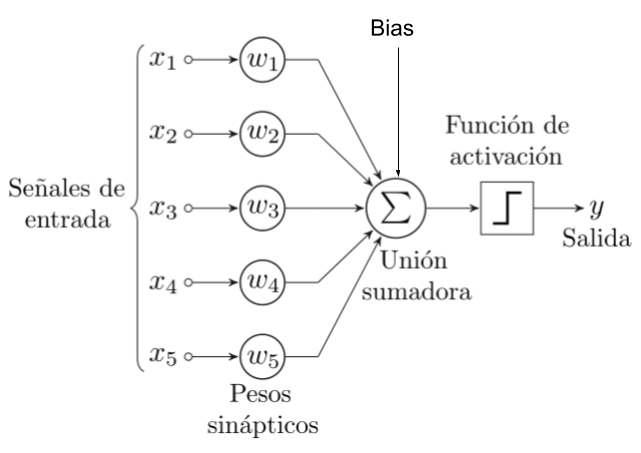
\includegraphics[width=0.4\textwidth]{img/perceptron.png}
    \caption{Modelo del perceptrón simple}
    \label{img: perceptron}
\end{figure}

La primera etapa del proceso consiste en calcular la suma promediada de sus entrada mediante una función lineal
\begin{equation}
f(x) = \sum_{i=1}^{n} w_i \cdot x_i + b
\end{equation}
Los coeficientes $w_i$, $i=1,2, \ldots, n$ llamados pesos, dan un valor determinado a cada una de las entradas en función de la importancia para obtener la salida. Además, el coeficiente $b$ es el sesgo o bias que se añade a la función. Otra forma práctica de escribir esta ecuación sería: $f(x) = \sum_{i=1}^{n+1} w_i \cdot z_i = w^t\cdot z  donde w = (w_1, \ldots, w_n, b)^t y z^t = (x_1, \ldots, x_n, 1)^t$

La segunda capa consiste en transformar la salida de la primera etapa mediante una función de activación. En el caso de un problema de clasificación binaria (0 o 1), si esta salida sobrepasa un cierto umbral predefinido al principio, su salida será 1 y en caso contrario, será 0. Es decir, siendo $c$ una constante real:

\begin{equation}
\text{y} = 
\begin{cases} 
1  \text{  si  }  \sum_{i=1}^{n} w_i \cdot x_i + b > c\\
0  \text{  si  }  \sum_{i=1}^{n} w_i \cdot x_i + b <= c.
\end{cases}
\end{equation}












\section{GENERALIZACIÓN}
\section{COMO SE APRENDE}
\section{OPTIMIZACIÓN}
\section{FUNCIÓN DE PERDIDA}
\section{FUNCION DE ACTIVACION}
\section{VALIDACIÓN CRUZADA}
\section{ARQUITECTURAS}
\section{REGULARIZACIÓN}
\section{MÉTRICAS}
\section{FRAMEWORKS}






\section{Arquitecturas relevantes} \label{Subsec: 3_2}
Mini tabla resumen en Deep Cybersecurity: A Comprehensive Overview from Neural Network and Deep Learning Perspective y miniresumen de todos los tipos en review Deep Cybersecurity: A Comprehensive Overview from Neural Networkand Deep Learning Perspective y review

\subsection{Autoencoder}

Los autoencoders son una clase de redes neuronales artificiales utilizadas en aprendizaje no supervisado para aprender representaciones eficientes de los datos. Su funcionamiento consiste en codificar la entrada en una representación comprimida y significativa, y luego decodificarla de manera que la reconstrucción sea lo más similar posible a la entrada original \citep{lopes2022effective}. La arquitectura básica de un autoencoder consta de tres partes: el encoder, el cuello de bottela y el decoder (Figura \ref{fig:AE_architecture}). 

\begin{figure}[h]
    \centering
    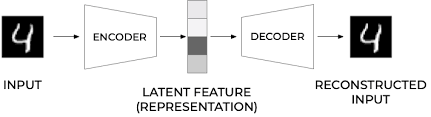
\includegraphics[width=0.6\textwidth]{img/AE4.png}
    \caption{Arquitectura de un autoencoder. Fuente:\citep{autoencoderImage}.}
    \label{fig:AE_architecture}
\end{figure}

El encoder mapea los datos de entrada a una representación oculta de menor dimensión utilizando funciones principalmente no lineales, mientras que el decoder reconstruye los datos de entrada a partir de esta representación oculta. Durante el entrenamiento, los parámetros del autoencoder se optimizan para minimizar la diferencia entre la entrada y la salida reconstruida, utilizando una función de pérdida que mide esta discrepancia, como por ejemplo la pérdida de entropía cruzada. Esto concluye el proceso de entrenamiento de un autoencoder.


El problema, tal como se define formalmente en \cite{bank2023autoencoders}, es aprender las funciones
\[
A : \mathbb{R}^n \rightarrow \mathbb{R}^p \quad \text{(encoder)}
\]
y
\[
B : \mathbb{R}^p \rightarrow \mathbb{R}^n \quad \text{(decoder)}
\]
que satisfacen
\[
\arg \min_{A, B} \mathbb{E}[\Delta(x, B \circ A(x))],
\]
donde $\mathbb{E}$ es la esperanza sobre la distribución de $x$, y $\Delta$ es la función de pérdida de reconstrucción, que mide la distancia entre la salida del decodificador y la entrada.


Las ecuaciones para obtener la salida de un autoencoder serían:
\[
\left\{
\begin{aligned}
z^{(1)} &= W^{(1)} \cdot x + b^{(1)} \\
a^{(2)} &= f(z^{(1)})  \\
z^{(2)} &= W^{(2)} \cdot a^{(2)} + b^{(2)}  \\
y &= z^{(2)} 
\end{aligned}
\right.
\]

donde  $x$ es el input, \( b^{(1)} \) y  \( b^{(2)} \) son los sesgos,  \( W^{(1)} \) y  \( W^{(2)} \) son los pesos, \( z^{(1)} \) es la salida lineal de la primera capa, \( a^{(2)} \) es la activación de la segunda capa, \( z^{(2)} \) es la salida lineal de la segunda capa e \( y \) es la salida final del modelo \citep{martinez2017analisis}.


Los autoencoders se utilizan en una amplia variedad de aplicaciones, incluida la reducción de dimensionalidad, la extracción de características, la eliminación de ruido en los datos de entrada y la detección de anomalías. Su versatilidad y capacidad para aprender representaciones útiles de los datos los hacen herramientas poderosas.


Las principales capas que se utilizan en esta red neuronal son las capas densas y las de aplanamiento, aunque también se pueden utilizar capas convolucionales y de pooling para autocodificadores convolucionales\footnote{Autocodificador para imágenes de gran tamaño} o LSTM en el caso de autocodificadores recurrentes\footnote{Autocodificador específico para series temporales o secuencias.}\citep{geron2022hands}. 






\subsection{Deep Belief Networks}
\subsubsection{Red Neuronal Profunda}
\subsection{Red Neuronal Convolucional} \label{sec:2.CNN}


Las redes neuronales convolucionales son una de las métodos de machine learning más importantes y utilizados en el campo de la ciberseguridad. Estas redes neuronales están diseñadas para procesar entradas almacenadas en matrices, como las imágenes.  Son una parte de las redes profundas que procesa y analiza entradas de imágenes visuales, y están compuestas por neuronas con pesos y sesgos que aprenden a lo largo de su entrenamiento \citep{podder2021artificial}. La arquitectura de una CNN (Figura \ref{fig:cnn_architecture}) consta de tres tipos de capas: capas de convolución, capas de pooling y la capa de clasificación. 
 

\begin{figure}[h]
    \centering
    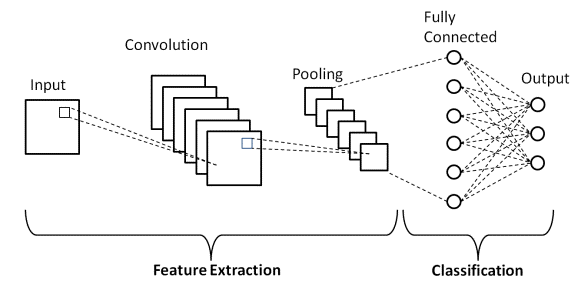
\includegraphics[width=0.6\textwidth]{img/convlayers.png}
    \caption{Arquitectura de una CNN con capas de convolución, pooling y clasificación. Fuente:\citep{phung2018deep}.}
    \label{fig:cnn_architecture}
\end{figure}

\subsubsection*{Capas convolucionales}

La capa convolucional es la capa más importante de una \acrshort{cnn}. En ella se extraen las características más significativas de la imagen de entrada, como los bordes, el color o la forma. Para ello se aplica una convolución a la imagen con un filtro. Esta operación matemática se representa como \( \int (x \star w)(t) \) donde $x$ representa la entrada y $w$ el núcleo de convolución \citep{pajares2021aprendizaje}.



En una CNN, la entrada de la convolución es una matriz multidimensional mientras que $w$ es una matriz de parámetros, llamada núcleo o filtro, que se ajusta durante el aprendizaje.
Cada píxel de la capa de convolución tiene una neurona, que se conecta con la capa anterior aplicando la convolución con las neuronas de su campo receptivo\footnote{Región de entrada que contribuye a la salida generada por el filtro} \cite{geron2022hands}. Esta convolución se realiza con un solapamiento total del filtro, lo que resulta en una imagen de menor dimensión (Figura \ref{fig:convolucion}). Si se desea mantener la misma dimensión, se puede aplicar zero-padding, que consiste en rellenar con ceros la matriz para obtener las dimensiones deseadas (Figura \ref{fig:convolucionPadding}). En la figura \ref{fig:convolu2} se muestran sendos campos receptivos de la imagen \( I \) que contribuyen a las salidas \( P \) y \( Q \) generadas por el filtro \( K \). La matriz de respuesta al aplicarle el kernel se llama mapa de características.

\begin{figure}[h] 
     \centering
     \begin{subfigure}[b]{0.45\textwidth}
         \centering
         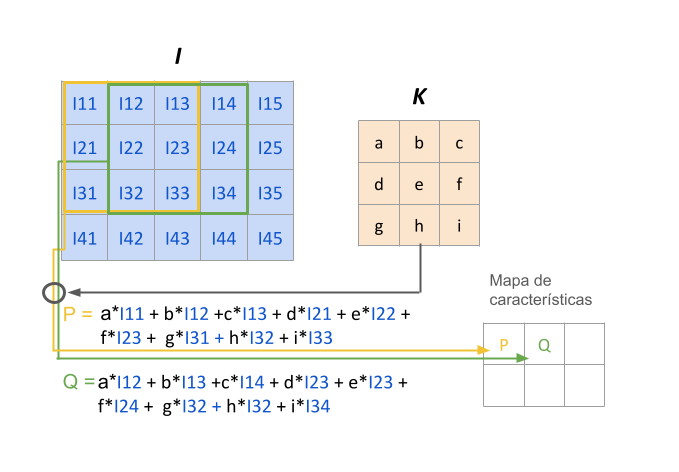
\includegraphics[width=\textwidth]{img/convolucion.png}
         \caption{Convolución reduciendo tamaño.}
         \label{fig:convolucion}
     \end{subfigure}
     \hfill
     \begin{subfigure}[b]{0.45\textwidth}
         \centering
         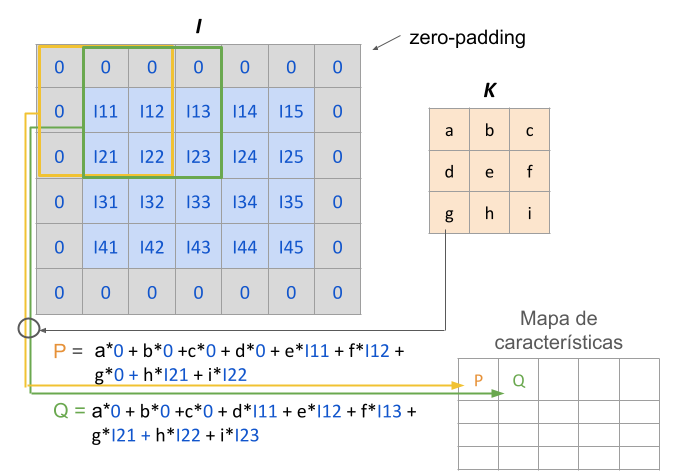
\includegraphics[width=1\textwidth]{img/convolucionPadding.png}
         \caption{Convolución con zero-padding.}
         \label{fig:convolucionPadding}
     \end{subfigure}
     \caption{Convolución en 2D.}
     \label{fig:convolu2}
\end{figure} 

Se observa que el filtro se desplaza por la matriz \textit{I} con paso unitario en vertical y horizontal. Este parámetro se llama stride y su valor depende de el objetivo que se quiera lograr con esta capa convolucional.

\begin{figure}[h]
    \centering
    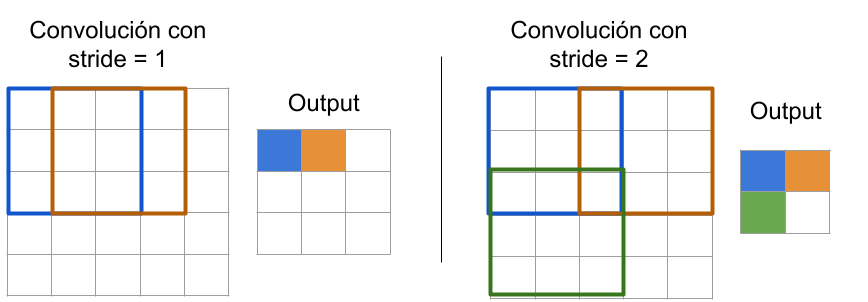
\includegraphics[width=0.6\textwidth]{img/stride.png}
    \caption{Campos receptivos en una convolución. Adaptación de imagen de \citep{yepez2020stride}}
    \label{fig:receptive_field}
\end{figure}

Una longitud de paso de 1 se utiliza normalmente para extraer el máximo número de características, ya que proporciona el máximo solapamiento entre el núcleo y la entrada. Por otro lado, cuando la longitud de paso es mayor que 1, los campos receptivos se solapan menos y producen una salida más pequeña. Si la longitud de paso fuera 3, habría problemas con el espaciado, ya que el campo receptivo no encajaría alrededor de la entrada como un número entero \citep{yepez2020stride}.



Por simplicidad, se ha usado siempre un único kernel, pero se puede generalizar a varios filtros, creando un mapa de características por cada uno. En cada uno de estos mapas hay una neurona por pixel y todas ellas comparten los mismos parámetros, lo que reduce considerablemente el número de parámetros del modelo. El campo receptivo de una neurona ahora se extiende por los mapas de características de todas las capas anteriores \citep{geron2022hands}.



Toda la información anterior se resume en la siguiente ecuación \citep{pajares2021aprendizaje}:

\begin{equation}
z_{i,j,k} = b_k + \sum_{u=0}^{f_h-1} \sum_{v=0}^{f_w-1} \sum_{k'=0}^{f_n'-1} x_{i',j',k'} \cdot w_{u,v,k',k} \hspace{5mm} \textup{con }
\left\{
\begin{array}{l}
i' = i \cdot s_h + u \\
j' = j \cdot s_w + v
\end{array}
\right.
\end{equation}

donde:
\begin{itemize}
    \item \( z_{i,j,k} \) es la salida de la neurona ubicada en la fila \(i\), columna \(j\) en el mapa de características \(k\) de la capa convolucional (capa \(l\)).
    \item \( s_h \) y \( s_w \) son los pasos de avance vertical y horizontal.
    \item \( f_h \) y \( f_w \) son la altura y la anchura del campo receptivo y \( f_{n'} \) es el número de mapas de características de la capa anterior (capa \(l-1\)).
    \item \( x_{i',j',k'} \) es la salida de la neurona situada en la fila \(i'\), columna \(j'\), mapa de características \(k'\).
    \item \( b_k \) es el sesgo para el mapa de características \(k\) (en la capa \(l\)).
    \item \( w_{u,v,k',k} \) es el peso de conexión entre cualquier neurona del mapa de características \(k\) de la capa \(l\) y su entrada situada en la fila \(u\), columna \(v\) (relativa al campo receptivo de la neurona) y el mapa de características \(k'\).
\end{itemize}





\subsubsection*{Capas de pooling}

El siguiente tipo de capa de las \acrshort{cnn} son las pooling, cuyo objetivo es reducir la imagen de entrada para disminuir la carga computacional, el uso de memoria y el número de parámetros, limitando así el riesgo de sobreajuste y proporcionando robustez contra el ruido y las distorsiones. Esta capa se suele colocar entre las capas de convolución, permitiendo reducir el tamaño de las imágenes mientras se preservan las características más importantes \citep{podder2021artificial}. Al igual que en las capas convolucionales, sus neuronas están conectadas a un pequeño grupo de neuronas de la capa anterior a las que se le aplica una función de agregación\footnote{Las funciones de agregación devuelven un valor único de un conjunto de registros.}. Las tres funciones más comunes son el promedio, la suma y el máximo. La Figura \ref{fig:maxpooling} muestra una capa de max pooling, que es el tipo más común \citep{geron2022hands}. 



\begin{figure}[h!]
\centering
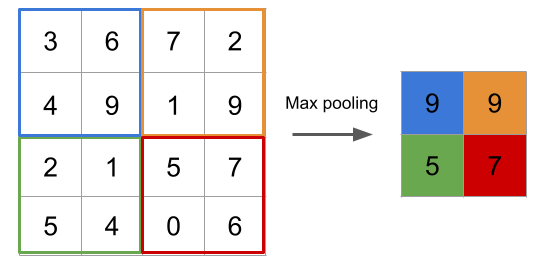
\includegraphics[width=0.4\textwidth]{img/maxpooling.png}
\caption{Capa de max pooling con un kernel de \( 2 \times 2 \), stride 2 y sin padding.}
\label{fig:maxpooling}
\end{figure}

Además de reducir el número de operaciones, el número de parámetros y ayudar con el overfitting, una capa de max pooling introduce cierto nivel de invarianza a pequeñas translaciones, ya que si un pixel se traslada hacia la derecha, la salida también debería trasladarse un pixel hacia la derecha, como se ilustra en la Figura \ref{fig:translacionPooling}. Esto significa que pequeñas variaciones en la posición de las características dentro de la imagen no afectan significativamente la salida.


\begin{figure}[h!]
\centering
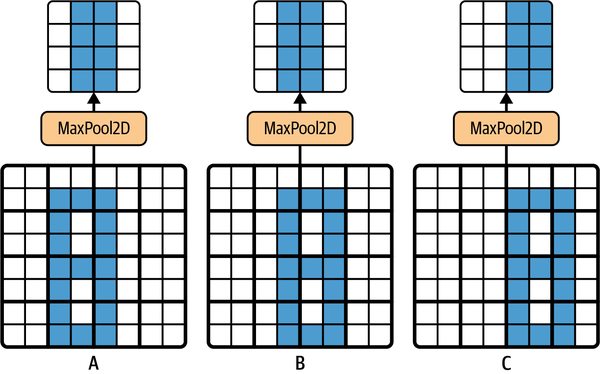
\includegraphics[width=0.4\textwidth]{img/translacionPooling.png}
\caption{Invarianza a translaciones pequeñas mediante una capa de max pooling. Fuente \citep{geron2022hands}}
\label{fig:translacionPooling}
\end{figure}



\subsubsection*{Capas Totalmente Conectadas (Fully Connected)}

Por último están las capas totalmente conectadas (\textit{fully connected}), que realizan la clasificación sobre la salida generada por las capas de convolución y pooling. Como el input de una capa densa debe ser un vector, primero se debe aplanar la salida de la última capa para poder utilizar después esta capa. Cada una de sus neuronas está conectada a todas las de la capa anterior, estableciendo una red densa de conexiones. Este tipo de neuronas suele ir seguido de una capa Dropout para mejorar la generalización del modelo. Este diseño permite a las CNN manejar datos complejos y variados, aprovechando la jerarquía de características aprendidas durante el entrenamiento. Este tipo de capa suele ir seguido de una capa de Dropout que mejora la capacidad de generalización del modelo al prevenir el sobreajuste, un problema común en el ámbito del aprendizaje profundo \citep{hossain2019classification}.


\begin{comment}
%Adicionalmente, las CNN pueden utilizar técnicas de regularización que ayudan a reducir el sobreajuste. Una de las técnicas más exitosas se llama \textit{dropout} \citep{srivastava2014dropout}. Al entrenar un modelo utilizando \textit{dropout}, durante cada iteración de entrenamiento, un porcentaje especificado de nodos en una capa dada y sus conexiones entrantes y salientes se eliminan aleatoriamente. Incluir \textit{dropout} típicamente mejora la precisión y la capacidad de generalización de un modelo porque aumenta la probabilidad de que un nodo sea útil.

\subsubsection{Aplicaciones y Éxitos}

Los usos de las CNN son significativamente variados. El mayor éxito se ha logrado en tareas de visión por computadora, como la detección y reconocimiento de objetos y escenas \citep{krizhevsky2012imagenet}. Las aplicaciones van desde la biología \citep{ronneberger2015u} hasta el reconocimiento facial \citep{parkhi2015deep}. El mejor ejemplo del éxito de las CNN tuvo lugar en 2012 en la competencia ImageNet, donde una CNN superó el rendimiento de otros métodos y luego la precisión humana en 2015 mediante el uso de GPUs, ReLUs, \textit{dropout} y la generación de imágenes adicionales \citep{he2015delving}. Además, las CNN se han utilizado con éxito en modelos de lenguaje para la detección de fonemas \citep{hinton2012deep}, reconocimiento de letras \citep{lecun1998gradient}, reconocimiento de voz \citep{graves2013speech} y construcción de modelos de lenguaje \citep{collobert2008unified}.



Una de las redes neuronales más importantes y más utilizadas en el campo de la ciberseguridad son la \acrfull{cnn}. Las CNN tienen su origen en el estudio de la corteza visual del cerebro y han sido utilizadas en el reconocimiento de imágenes desde la década de los 80. Actualmente, debido al aumento en la capacidad computacional, la disponibilidad de grandes volúmenes de datos de entrenamiento y las técnicas avanzadas de redes profundas, han permitido que las CNN alcancen un rendimiento excepcional en tareas visuales complejas. Estas redes son la base de servicios como la búsqueda de imágenes o los vehículos autónomos. Además, las CNN no se limitan únicamente a la percepción visual, también han demostrado ser efectivas en tareas como el reconocimiento de voz y el procesamiento del lenguaje natural \citep{geron2022hands}. No obstante, nos enfocaremos únicamente en sus aplicaciones visuales.

\end{comment}

\subsection{Red Neuronal Recurrente}
\subsubsection{Restricted Boltzmann Machine}









\section{Bibliotecas utilizadas en Python} \label{Subsec: 3_3}

Para nuestros experimentos, utilizaremos Python debido a su popularidad y versatilidad en el ámbito del aprendizaje automático y la inteligencia artificial. Python ofrece una amplia gama de bibliotecas especializadas que facilitan la creación, entrenamiento y evaluación de modelos, así como el análisis y visualización de datos. A continuación, se describen las principales bibliotecas y frameworks que emplearemos en este trabajo, destacando sus características y ventajas.


\subsection{Principales frameworks. Keras}

Como las técnicas de aprendizaje profundo han ido ganando popularidad, muchas organizaciones académicas e industriales se han centrado en desarrollar marcos para facilitar la experimentación con redes neuronales profundas. En esta sección, ofrecemos una visión general de los marcos de trabajo más importantes que se pueden usar en Python, concluyendo con nuestra elección.


\textbf{TensorFlow} \citep{tensorflow} es una biblioteca de código abierto desarrollada por el equipo de Google Brain para la computación numérica y el aprendizaje automático a gran escala. Diseñada para ser altamente flexible, TensorFlow soporta computación distribuida y permite la optimización de gráficos computacionales, lo que mejora significativamente la velocidad y el uso de memoria de las operaciones. En su núcleo, TensorFlow es similar a NumPy pero con soporte para GPU, lo que acelera considerablemente los cálculos. Además, incluye herramientas avanzadas como TensorBoard para la visualización de modelos y TensorFlow Extended para la producción de modelos de aprendizaje automático. Gracias a estas capacidades, TensorFlow se ha convertido en una herramienta esencial en la industria y la investigación, siendo utilizada en aplicaciones que van desde la clasificación de imágenes y el procesamiento de lenguaje natural hasta los sistemas de recomendación y la previsión de series temporales.


\textbf{Keras} \citep{keras} es una API de alto nivel para redes neuronales que ahora es parte integral de TensorFlow. Fue desarrollada por François Chollet y ganó popularidad rápidamente gracias a su simplicidad y diseño elegante. Inicialmente, Keras soportaba múltiples backends, pero desde la versión 2.4, funciona exclusivamente con TensorFlow \citep{muller2016introduction}. Keras permite a los usuarios construir, entrenar y evaluar modelos de aprendizaje profundo de manera rápida y eficiente. Su facilidad de uso y extensa documentación la convierten en una herramienta valiosa tanto para la investigación como para la implementación de aplicaciones de inteligencia artificial.



\textbf{PyTorch} \citep{pytorch}, desarrollado por el equipo de investigación de IA de Facebook, es una biblioteca de aprendizaje profundo que destaca por su enfoque en la computación dinámica, lo que permite una mayor flexibilidad en la creación de modelos complejos. A diferencia de TensorFlow, que utiliza gráficos computacionales estáticos, PyTorch permite que la topología de la red neuronal cambie durante la ejecución del programa \citep{mahmoud2019dlbench}. Esto, junto con su capacidad de auto-diferenciación en modo inverso\footnote{Técnica en la que PyTorch calcula automáticamente las derivadas de las funciones de pérdida con respecto a los parámetros del modelo.}, hace que PyTorch sea popular entre los investigadores y desarrolladores. Su facilidad de uso y robusta comunidad de apoyo han llevado a su adopción por parte de importantes organizaciones como Facebook, Twitter y NVIDIA.



Para escoger con cuál de estas librerías se realizará la parte práctica de este trabajo, vamos a utilizar, además de las características previamente vistas, los resultados de \citep{mahmoud2019dlbench}. En él se hace un estudio de eficiencia, convergencia, tiempo de entrenamiento y uso de memoria de los diferentes frameworks con varios datasets. Entre sus resultados podemos observar como Keras destaca por encima de las demás en el entorno de la CPU. No solo logra el mejor accuracy en los tres datasets (MNIST, CIFAR-10, CIFAR-100), sino que además también tiene los tiempos de ejecución más bajos y una de las mejores tasas de convergencia. En cuento al entorno de la GPU, las tres librerías obtienen unos resultados semejantes. En conclusión, podemos afirmar que estos resultados junto con su facilidad de uso, accesibilidad y documentación bien estructurada, han sido determinantes para optar por usar Keras en vez de PyTorch o TensorFlow en nuestros estudios posteriores. Aakash Nain resume perfectamente las ventajas de Keras \citep{keraswebsite2} al señalar que:

\begin{quote} 
``Keras is that sweet spot where you get flexibility for research and consistency for deployment. Keras is to Deep Learning what Ubuntu is to Operating Systems.'' 
\end{quote}

De manera similar, Matthew Carrigan destaca la intuitividad y facilidad de uso de Keras \citep{keraswebsite}, afirmando:

\begin{quote}
``The best thing you can say about any software library is that the abstractions it chooses feel completely natural, such that there is zero friction between thinking about what you want to do and thinking about how you want to code it. That's exactly what you get with Keras.''
\end{quote}


\subsection{Librerías y herramientas esenciales.} \label{sec:2.3.2}

De forma complementaria, también es importante conocer y utilizar diversas librerías y herramientas esenciales que facilitan el desarrollo y análisis de los modelos de Keras. Estas incluyen herramientas para la manipulación, visualización y análisis de datos.

\textbf{Scikit-Learn} \citep{scikitlearn} es una librería de código abierto con herramientas simples y eficientes para el análisis predictivo de datos. Contiene varios algoritmos de aprendizaje automático, desde clasificación y regresión hasta clustering y reducción de dimensionalidad, con la documentación completa sobre cada algoritmo. Está construida sobre otras librerías que veremos más adelante como Numpy, SciPy y matplotlib. Aunque no se aprovecharán todas estas funcionalidades de scikit-learn, si que se va a utilizar una de sus funciones más populares, \texttt{train\_test\_split()} \citep{traintestsplit}. Esta función divide el dataset en dos subconjuntos de forma aleatoria, manteniendo la correspondencia en caso de que el dataset contenga dos o más partes. Usualmente, a estos subconjuntos se les llama conjunto de prueba y conjunto de entrenamiento, cuyo tamaño se indica con un valor entre 0 y 1 (\texttt{test\_size}). Además, también se suele asignar una semilla a esa división para que cada vez que se quieran reproducir los experimentos, pueda usarse la misma partición. Esa semilla es un número natural que se introduce como parámetro de entrada en la variable \texttt{random\_state}. Veamos un ejemplo de como utilizar esta función.


\lstset{language=Python}
\begin{lstlisting}
# Ejemplo de codigo en Python
from sklearn.model_selection import train_test_split

X_train, X_test, y_train, y_test = train_test_split(data, labels,
                                        test_size=0.25, random_state=42)
\end{lstlisting}


Las variables X\_train, X\_ test y compañía son numpy arrays. \textbf{NumPy} \citep{numpy} es el paquete fundamental de Python para la computación científica. Es una biblioteca general de estructuras de datos, álgebra lineal y manipulación de matrices para Python, cuya sintaxis y manejo de estructuras de datos y matrices es comparable al de MATLAB \citep{bloice2016tutorial}. En NumPy, se pueden crear arrays y realizar operaciones rápidas y eficientes sobre ellos. Se utilizarán estas estructuras de datos para almacenar los datos y entrenar las redes neuronales con ellas. Aunque también se pueden utilizar tensores \citep{modeltraining}, se ha decidido utilizar numpy arrays por su alta eficiencia operacional y por su uso en la industria.


Otro paquete que se va a utilizar durante los experimentos y que Scikit-Learn utiliza es \textbf{matplotlib} \citep{matplotlib}. Es la principal biblioteca de gráficos científicos en Python y proporciona funciones para crear visualizaciones de calidad como gráficos de barras, histogramas, gráficos de dispersión, etc. Se utilizará este paquete para representar gráficamente los datos de cada dataset para poder obtener bastante información con un simple vistazo. 












\begin{comment}
¿QUITAR?
La ecuación \ref{eq:conv} resume las explicaciones anteriores en una gran ecuación matemática \citep{pajares2021aprendizaje}:

\begin{equation}
z_{i,j,k} = b_k + \sum_{u=0}^{f_h-1} \sum_{v=0}^{f_w-1} \sum_{k'=0}^{f_n'-1} x_{i',j',k'} \cdot w_{u,v,k',k} \hspace{5mm} \textup{con }
\left\{
\begin{array}{l}
i' = i \cdot s_h + u \\
j' = j \cdot s_w + v
\end{array}
\right.
\end{equation} \label{eq:conv}

donde \( z_{i,j,k} \) es la salida de la neurona ubicada en \((i,j)\) en el mapa de características \(k\) de la capa convolucional \(l\). \( s_h \) y \( s_w \) es el stride vertical y horizontal. \( f_h \) y \( f_w \) son las dimensiones del campo receptivo y \( f_{n'} \) es el número de mapas de características de la capa anterior. \( x_{i',j',k'} \) es la salida de la neurona situada en \((i',j')\) y en mapa de características \(k'\). \( b_k \) es el término de sesgo para el mapa de características \(k\) en la capa \(l\) y \( w_{u,v,k',k} \) es el peso de conexión entre cualquier neurona del mapa de características \(k\) de la capa \(l\) y su entrada en \((u,v)\) y el mapa de características \(k'\).
\end{comment}



\begin{comment}
Una de las redes neuronales más importantes y más utilizadas en el campo de la ciberseguridad son las \acrfull{cnn}. Las CNN tienen su origen en el estudio de la corteza visual del cerebro y han sido utilizadas en el reconocimiento de imágenes desde la década de los 80. Actualmente, debido al aumento en la capacidad computacional, la disponibilidad de grandes volúmenes de datos de entrenamiento y las técnicas avanzadas de redes profundas, han permitido que las CNN alcancen un rendimiento excepcional en tareas visuales complejas. Estas redes son la base de servicios como la búsqueda de imágenes o los vehículos autónomos \citep{geron2022hands}.


Una \acrfull{cnn} es una red neuronal diseñada para procesar entradas almacenadas en matrices. Un ejemplo de entrada es una imagen en escala de grises, que es una matriz bidimensional (2D) de píxeles. Aunque estas redes se utilicen principalmente en la clasificación visual de imágenes, también  se han demostrado que son efectivas en tareas como el reconocimiento de voz (matrices 2D de imágenes o espectrogramas de audio) \citep{kim2023bilstm}, clasificación visual de videos o imágenes volumétricas (matrices tridimensionales 3D) \citep{diba2017temporal} y procesamiento de lenguaje natural(matriz 2D) \citep{wang2017combining}. Independientemente de la dimensionalidad, las CNN se utilizan donde hay un ordenamiento espacial o temporal \citep{berman2019survey}. No obstante, nos enfocaremos únicamente en sus aplicaciones visuales.

La arquitectura de una CNN (ver Figura ????????) consta de tres tipos distintos de capas: capas de convolución, capas de pooling y la capa de clasificación. 

IMAGEN CAPAS: \citep{phung2018deep}


\subsubsection*{Capas convolucionales}

La capa convolucional es el bloque de construcción más importante de una red neuronal convolucional (CNN). En ella se aplica la operación de convolución, que involucra dos funciones y produce una tercera función que representa la cantidad de superposición de una función a medida que se desplaza sobre otra. Supóngase que se tiene una fuente de luz variable cuya intensidad se recibe mediante un sensor. Este sensor proporciona una salida en una determinada posición \( x \) en el tiempo \( t \), esto es, \( x(t) \). Tanto \( x \) como \( t \) son valores reales, de forma que debido a la variabilidad de la fuente mencionada, se pueden obtener diferentes lecturas en diferentes instantes de tiempo. La captura de la señal por el sensor puede estar contaminada con cierto ruido. Para obtener una señal más limpia, lo acertado es realizar un promediado de la salida con varias medidas. Si además tenemos en cuenta que las medidas más recientes son más relevantes que las alejadas en el tiempo, el promediado puede ponderarse concediendo más relevancia a las medidas recientes. Esto puede hacerse mediante una función de promediado \( w(a) \), donde \( a \) representa el alejamiento de la medida en el tiempo. Si se realiza esta operación de promediado ponderado en cada instante de tiempo \( t \), se obtiene una nueva función promediada como sigue:

\begin{equation}
s(t) = \int x(a) w(t-a) \, da
\end{equation}

Esta operación se denomina convolución, y se denota como:

\begin{equation}
s(t) = \int (x \star w)(t)
\end{equation}

Para que el promedio ponderado sea válido, la función de promediado \( w(t) \) necesita ser una función de densidad de probabilidad. Además, \( w(t) \) debe ser cero para todos los valores negativos de \( t \) para evitar tomar valores futuros, lo cual no es físicamente posible \citep{pajares2021aprendizaje}.


Para aplicaciones prácticas como el procesamiento de imágenes, las medidas suelen ser discretas, es decir, se toman en intervalos de tiempo específicos. En este caso, el tiempo \( t \) toma valores enteros, y la convolución discreta se define como:

\begin{equation}
s(t) = (x \star w)(t) = \sum_{a=-\infty}^{\infty} x(a) w(t-a)
\end{equation}

En el contexto de las CNN, la entrada es un vector o matriz multidimensional de datos (la imagen), y el núcleo es una matriz multidimensional de parámetros que se ajustan durante el proceso de aprendizaje. Sea \( I \) la imagen de entrada y \( K \) un núcleo de convolución. Se define la convolución discreta en dos dimensiones como:

\begin{equation}
S(i, j) = (K \star I)(i, j) = \sum_{m=0}^{M-1} \sum_{n=0}^{N-1} I(i+m, j+n) K(m, n)
\end{equation}

donde \( M \) y \( N \) son las dimensiones del núcleo. La figura ????? muestra un ejemplo de convolución con el núcleo \( K \), aplicado sobre una imagen \( I \). 


En una CNN, esta construcción es la mas importante. Las neuronas de la primera capa convolucional se concectan a todos y cada uno de los píxeles de la imagen de entrada, sino solo a píxeles en sus campos receptivos. A su vez, cada neurona de la segunda capa convolucional está conectada a las neuronas ubicadas dentro de un rectángulo pequeño en la primera capa. Esta arquitectura permite a la red concentrarse en cracterísticas pequeñas de bajo nivel en la primera capa oculta, juntarlas después para crear características más grandes de nivel superior en la siguiente capa oculta, y así sucesivamente. La convolución se realiza con solapamiento total del núcleo, lo que resulta en una imagen resultante de menor dimensión (REFERENCIA IMAGEN A ?????). Si se desea mantener la misma dimensión, se puede aplicar relleno con ceros o zero-padding (REFERENCIA IMAGEN A ?????). Este relleno se indica como "same" en términos de implementación. Si no se realiza relleno con ceros, se indica como "valid". Por otra parte, en las convoluciones, el campo receptivo se define como la región de entrada que contribuye a la salida generada por el filtro. En la figura REFERENCIA IMAGEN A ?????) se muestran sendos campos receptivos de la imagen \( I \) que contribuyen a las salidas \( P \) y \( \Q \) generadas por el filtro \( K \).


IMAGENES PADDING

Por último, se define el stride. Stride es la longitud de paso de desplazamiento del núcleo alrededor de la entrada. Cuando la longitud de paso es 1, el núcleo se desplaza sobre la entrada un elemento a la vez. Normalmente, la longitud de paso se establece de manera que el volumen de salida sea un número entero.

FOTOOO stride Fuente:\citep{yepez2020stride}

La Figura de la izquierda muestra una entrada de \(5 \times 5\) con un núcleo de \(3 \times 3\). Con un stride de paso 1, se genera una matriz de salida de tamaño \(3 \times 3\). Una longitud de paso de 1 se utiliza normalmente para extraer el máximo número de características, ya que proporciona el máximo solapamiento entre el núcleo y la entrada, pero a máxima complejidad computacional. Por otro lado, la imagen de la derecha muestra el núcleo desplazándose dos unidades sobre la entrada, generando una matriz de salida de \(2 \times 2\). Generalmente, cuando la longitud de paso es mayor que 1, los campos receptivos se solapan menos y producen una salida más pequeña. Si la longitud de paso fuera 3, habría problemas con el espaciado, ya que el campo receptivo no encajaría alrededor de la entrada como un número entero \citep{yepez2020stride}.









cada neurona en la capa convolucional está conectada solo a una pequeña región de la imagen de entrada (campo receptivo). Estas conexiones se realizan utilizando filtros (o núcleos de convolución), y la salida se conoce como mapa de características. La ecuación \ref{eq:conv} resume las explicaciones anteriores en una gran ecuación matemática \citep{pajares2021aprendizaje}:

\begin{equation}
z_{i,j,k} = b_k + \sum_{u=0}^{f_h-1} \sum_{v=0}^{f_w-1} \sum_{k'=0}^{f_n'-1} x_{i',j',k'} \cdot w_{u,v,k',k} \hspace{5mm} \textup{con }
\left\{
\begin{array}{l}
i' = i \cdot s_h + u \\
j' = j \cdot s_w + v
\end{array}
\right.
\end{equation}

donde:
\begin{itemize}
    \item \( z_{i,j,k} \) es la salida de la neurona ubicada en la fila \(i\), columna \(j\) en el mapa de características \(k\) de la capa convolucional (capa \(l\)).
    \item \( s_h \) y \( s_w \) son los pasos de avance vertical y horizontal.
    \item \( f_h \) y \( f_w \) son la altura y la anchura del campo receptivo y \( f_{n'} \) es el número de mapas de características de la capa anterior (capa \(l-1\)).
    \item \( x_{i',j',k'} \) es la salida de la neurona situada en la fila \(i'\), columna \(j'\), mapa de características \(k'\) (o canal \(k'\) si la capa anterior es la capa de entrada).
    \item \( b_k \) es el término de sesgo para el mapa de características \(k\) (en la capa \(l\)). Puedes imaginarlo como una rueda que ajusta el brillo general del mapa de características \(k\).
    \item \( w_{u,v,k',k} \) es el peso de conexión entre cualquier neurona del mapa de características \(k\) de la capa \(l\) y su entrada situada en la fila \(u\), columna \(v\) (relativa al campo receptivo de la neurona) y el mapa de características \(k'\).
\end{itemize}









\subsection{Red Neuronal Convolucional}

Una de las redes neuronales más importantes y más utilizadas en el campo de la ciberseguridad son las \acrfull{cnn}. Las CNN tienen su origen en el estudio de la corteza visual del cerebro y han sido utilizadas en el reconocimiento de imágenes desde la década de los 80. Actualmente, debido al aumento en la capacidad computacional, la disponibilidad de grandes volúmenes de datos de entrenamiento y las técnicas avanzadas de redes profundas, han permitido que las CNN alcancen un rendimiento excepcional en tareas visuales complejas. Estas redes son la base de servicios como la búsqueda de imágenes o los vehículos autónomos \citep{geron2022hands}.

Una \acrfull{cnn} es una red neuronal diseñada para procesar entradas almacenadas en matrices. Un ejemplo de entrada es una imagen en escala de grises, que es una matriz bidimensional (2D) de píxeles. Aunque estas redes se utilicen principalmente en la clasificación visual de imágenes, también se ha demostrado que son efectivas en tareas como el reconocimiento de voz (matrices 2D de imágenes o espectrogramas de audio) \citep{kim2023bilstm}, clasificación visual de videos o imágenes volumétricas (matrices tridimensionales 3D) \citep{diba2017temporal} y procesamiento de lenguaje natural (matriz 2D) \citep{wang2017combining}. Independientemente de la dimensionalidad, las CNN se utilizan donde hay un ordenamiento espacial o temporal \citep{berman2019survey}. No obstante, nos enfocaremos únicamente en sus aplicaciones visuales.

La arquitectura de una CNN (ver Figura ????????) consta de tres tipos distintos de capas: capas de convolución, capas de pooling y la capa de clasificación.

\begin{figure}[h]
    \centering
    \includegraphics[width=0.8\textwidth]{path_to_image}
    \caption{Arquitectura de una CNN con capas de convolución, pooling y clasificación \citep{phung2018deep}.}
    \label{fig:cnn_architecture}
\end{figure}

\subsubsection*{Capas convolucionales}

La capa convolucional es el bloque de construcción más importante de una \fullacr{cnn}. En ella se aplica la operación de convolución, que involucra dos funciones y produce una tercera función que representa la cantidad de superposición de una función a medida que se desplaza sobre otra. Supóngase que se tiene una fuente de luz variable cuya intensidad se recibe mediante un sensor. Este sensor proporciona una salida en una determinada posición \( x \) en el tiempo \( t \), esto es, \( x(t) \). Tanto \( x \) como \( t \) son valores reales, de forma que debido a la variabilidad de la fuente mencionada, se pueden obtener diferentes lecturas en diferentes instantes de tiempo. La captura de la señal por el sensor puede estar contaminada con cierto ruido. Para obtener una señal más limpia, lo acertado es realizar un promediado de la salida con varias medidas. Si además tenemos en cuenta que las medidas más recientes son más relevantes que las alejadas en el tiempo, el promediado puede ponderarse concediendo más relevancia a las medidas recientes. Esto puede hacerse mediante una función de promediado \( w(a) \), donde \( a \) representa el alejamiento de la medida en el tiempo. Si se realiza esta operación de promediado ponderado en cada instante de tiempo \( t \), se obtiene una nueva función promediada como sigue:

\begin{equation}
s(t) = \int x(a) w(t-a) \, da
\end{equation}

Esta operación se denomina convolución, y se denota como:

\begin{equation}
s(t) = \int (x \star w)(t)
\end{equation}

Para que el promedio ponderado sea válido, la función de promediado \( w(t) \) necesita ser una función de densidad de probabilidad. Además, \( w(t) \) debe ser cero para todos los valores negativos de \( t \) para evitar tomar valores futuros, lo cual no es físicamente posible \citep{pajares2021aprendizaje}.


Para aplicaciones prácticas como el procesamiento de imágenes, las medidas suelen ser discretas, es decir, se toman en intervalos de tiempo específicos. En este caso, el tiempo \( t \) toma valores enteros, y la convolución discreta se define como:

\begin{equation}
s(t) = (x \star w)(t) = \sum_{a=-\infty}^{\infty} x(a) w(t-a)
\end{equation}

En el contexto de las CNN, la entrada es un vector o matriz multidimensional de datos (la imagen), y el núcleo es una matriz multidimensional de parámetros que se ajustan durante el proceso de aprendizaje. Sea \( I \) la imagen de entrada y \( K \) un núcleo de convolución. Se define la convolución discreta en dos dimensiones como:

\begin{equation}
S(i, j) = (K \star I)(i, j) = \sum_{m=0}^{M-1} \sum_{n=0}^{N-1} I(i+m, j+n) K(m, n)
\end{equation}

donde \( M \) y \( N \) son las dimensiones del núcleo. La figura \ref{fig:conv_example} muestra un ejemplo de convolución con el núcleo \( K \), aplicado sobre una imagen \( I \).

\begin{figure}[h]
    \centering
    \includegraphics[width=0.8\textwidth]{path_to_image}
    \caption{Ejemplo de convolución con un núcleo \( K \) aplicado sobre una imagen \( I \).}
    \label{fig:conv_example}
\end{figure}

En una CNN, esta construcción es la más importante. Las neuronas de la primera capa convolucional no se conectan a todos y cada uno de los píxeles de la imagen de entrada, sino solo a píxeles en sus campos receptivos. A su vez, cada neurona de la segunda capa convolucional está conectada a las neuronas ubicadas dentro de un rectángulo pequeño en la primera capa. Esta arquitectura permite a la red concentrarse en características pequeñas de bajo nivel en la primera capa oculta, juntarlas después para crear características más grandes de nivel superior en la siguiente capa oculta, y así sucesivamente. La convolución se realiza con solapamiento total del núcleo, lo que resulta en una imagen resultante de menor dimensión (ver Figura \ref{fig:padding_valid}). Si se desea mantener la misma dimensión, se puede aplicar relleno con ceros o zero-padding (ver Figura \ref{fig:padding_same}). Este relleno se indica como "same" en términos de implementación. Si no se realiza relleno con ceros, se indica como "valid". Por otra parte, en las convoluciones, el campo receptivo se define como la región de entrada que contribuye a la salida generada por el filtro. En la figura \ref{fig:receptive_field} se muestran sendos campos receptivos de la imagen \( I \) que contribuyen a las salidas \( P \) y \( Q \) generadas por el filtro \( K \).

\begin{figure}[h]
    \centering
    \includegraphics[width=0.8\textwidth]{path_to_image}
    \caption{Convolución con relleno "valid".}
    \label{fig:padding_valid}
\end{figure}

\begin{figure}[h]
    \centering
    \includegraphics[width=0.8\textwidth]{path_to_image}
    \caption{Convolución con relleno "same".}
    \label{fig:padding_same}
\end{figure}

\begin{figure}[h]
    \centering
    \includegraphics[width=0.8\textwidth]{path_to_image}
    \caption{Campos receptivos en una convolución.}
    \label{fig:receptive_field}
\end{figure}

Por último, se define el stride. Stride es la longitud de paso de desplazamiento del núcleo alrededor de la entrada. Cuando la longitud de paso es 1, el núcleo se desplaza sobre la entrada un elemento a la vez. Normalmente, la longitud de paso se establece de manera que el volumen de salida sea un número entero.

\begin{figure}[h]
    \centering
    \includegraphics[width=0.8\textwidth]{path_to_image}
    \caption{Ejemplo de convolución con diferentes strides. Fuente: \citep{yepez2020stride}.}
    \label{fig:stride_example}
\end{figure}

La Figura \ref{fig:stride_example} de la izquierda muestra una entrada de \(5 \times 5\) con un núcleo de \(3 \times 3\). Con un stride de paso 1, se genera una matriz de salida de tamaño \(3 \times 3\). Una longitud de paso de 1 se utiliza normalmente para extraer el máximo número de características, ya que proporciona el máximo solapamiento entre el núcleo y la entrada, pero a máxima complejidad computacional. Por otro lado, la imagen de la derecha muestra el núcleo desplazándose dos unidades sobre la entrada, generando una matriz de salida de \(2 \times 2\). Generalmente, cuando la longitud de paso es mayor que 1, los campos receptivos se solapan menos y producen una salida más pequeña. Si la longitud de paso fuera 3, habría problemas con el espaciado, ya que el campo receptivo no encajaría alrededor de la entrada como un número entero.



La ecuación \ref{eq:conv} resume las explicaciones anteriores en una gran ecuación matemática \citep{pajares2021aprendizaje}:

\begin{equation}
z_{i,j,k} = b_k + \sum_{u=0}^{f_h-1} \sum_{v=0}^{f_w-1} \sum_{k'=0}^{f_n'-1} x_{i',j',k'} \cdot w_{u,v,k',k} \hspace{5mm} \textup{con }
\left\{
\begin{array}{l}
i' = i \cdot s_h + u \\
j' = j \cdot s_w + v
\end{array}
\right.
\end{equation}

donde:
\begin{itemize}
    \item \( z_{i,j,k} \) es la salida de la neurona ubicada en la fila \(i\), columna \(j\) en el mapa de características \(k\) de la capa convolucional (capa \(l\)).
    \item \( s_h \) y \( s_w \) son los pasos de avance vertical y horizontal.
    \item \( f_h \) y \( f_w \) son la altura y la anchura del campo receptivo y \( f_{n'} \) es el número de mapas de características de la capa anterior (capa \(l-1\)).
    \item \( x_{i',j',k'} \) es la salida de la neurona situada en la fila \(i'\), columna \(j'\), mapa de características \(k'\) (o canal \(k'\) si la capa anterior es la capa de entrada).
    \item \( b_k \) es el término de sesgo para el mapa de características \(k\) (en la capa \(l\)).
    \item \( w_{u,v,k',k} \) es el peso de conexión entre cualquier neurona del mapa de características \(k\) de la capa \(l\) y su entrada situada en la fila \(u\), columna \(v\) (relativa al campo receptivo de la neurona) y el mapa de características \(k'\).
\end{itemize}
\end{comment}



\begin{comment}
Dentro del AA se encuadra el conocido como Aprendizaje Profundo (AP). En la literatura especializada a nivel internacional es muy común referirse al AP por sus términos en inglés, esto es, Deep Learning, que es el núcleo central del presente libro. Por otra parte, y al hilo de esta cuestión, conviene reseñar que son muchos y diversos los términos en inglés utilizados para definir y describir los conceptos involucrados bajo el paradigma del AP. Muchos de los cuales no poseen una clara traducción conceptual al español, razón por la cual los considerados bajo esta situación se mantienen a lo largo del libro con el fin de que el lector pueda fácilmente identificarlos en la literatura especializada escrita en inglés. Solo se han traducido aquellos conceptos que no admiten discusión, manteniendo en todo caso su expresión original en inglés.

Bien es cierto que desde los años 50 del siglo pasado, la IA a veces se ha sobrevalorado y se ha considerado como muy prometedora en diversas ocasiones, eso pese a que no se han llegado a alcanzar las perspectivas iniciales. Por otra parte, no es menos cierto que en los últimos años se están viendo avances importantes gracias al AP. Ello a pesar de que todavía es relativamente frágil de cara a su generalización y adaptación a entornos o escenarios cambiantes, principalmente por falta de datos suficientes que capturen los cambios de dicho entorno, pudiendo aparecer ciertos sesgos por falta de la información necesaria extraíble de los datos. Algunos autores como Marcus y Davis (2019), expresan, no sin cierta razón, algunos aspectos relativos a las ventajas e inconvenientes de los procesos de AP, achacándoles que muchas arquitecturas basadas en redes neuronales hacen cosas increíbles, sin ser conscientes por parte de quien las aplica del conocimiento real sobre lo que están haciendo, y por ello, no son sistemas totalmente inteligentes.

Aunque en parte, esto último puede verse desde esta perspectiva, no es menos cierto que los desarrollos basados en AP son capaces de conseguir resultados importantes, siendo esta la perspectiva desde la que se abordan y plantean los temas del presente libro.

Como sostienen Goodfellow y col. (2016), en los comienzos de la IA, se abordaron rápidamente problemas intelectualmente difíciles para los seres humanos, pero relativamente sencillos para las computadoras, todo ello mediante una lista de reglas matemáticas formales. A partir de ahí, el verdadero desafío para la IA se tornó en resolver tareas fáciles de realizar para las personas, pero difíciles de describir formalmente. Aquí se incluyen tareas tales como el reconocimiento de objetos en imágenes, palabras o acciones en los movimientos. No cabe duda de que en este aspecto el AP ha conseguido ya logros muy relevantes. Es en este rasgo, y más concretamente en la exposición de una serie de técnicas orientadas a tal fin, donde se centra el presente libro.

En definitiva, se trata de exponer una serie de técnicas para resolver problemas, por decirlo de alguna manera, intuitivos para el ser humano, con el uso de las computadoras, que aprenden mediante los métodos y algoritmos diseñados a partir de los datos suministrados y sin necesidad de que los humanos especifiquen formalmente todo el conocimiento requerido por la computadora. En cualquier caso, y siguiendo también la teoría expuesta en Goodfellow y col. (2016), la jerarquía de conceptos permite que la computadora aprenda conceptos complicados al construirlos a partir de otros más simples, todos ellos estructurados en múltiples capas, razón por la cual a este enfoque se le denomina con el término ya indicado de AP. En cualquier caso, como una técnica específica del AA, estos procedimientos se encaminan a extraer patrones determinados a partir de los datos.

Existe una diferencia fundamental en lo que respecta a la extracción de las mencionadas características entre las técnicas clásicas, por llamarlas de alguna manera, de AA y las específicas del AP. Por ejemplo, considérese un ejemplo sencillo biclase, en el que se trata de separar el cielo y la hierba en una imagen de color de un paisaje de campo. Los datos disponibles en este caso son valores de color de los píxeles, de forma que en el caso del cielo predominan las tonalidades azules, mientras que en la hierba son las verdes. Un método simple tal como naive Bayes puede separar los patrones en dos clases diferentes teniendo en cuenta que los mismos están definidos, por lo que se conoce como características. La extracción de características en este caso es esencial. Por otro lado, y siguiendo en el ámbito de las imágenes, estas se caracterizan por poseer información espacial, y en vídeos, también temporal. Las redes neuronales profundas pueden captar perfectamente ambos tipos de información. En el primer caso, los filtros de convolución son responsables de la captura espacial, a diferencia de lo que ocurre con otros modelos de red, tal como las de retropropagación, en las que las características de las imágenes se transforman en vectores que se suministran a la entrada, perdiendo las relaciones espaciales. Por ejemplo, una imagen de dimensión 3x3 se transforma en un vector con 9 componentes. En el caso de las características temporales las redes recurrentes tienen la habilidad de realizar tal captura.

No obstante, para muchas tareas no resulta fácil extraer características. Por ejemplo, supóngase que a partir de una imagen se quieren identificar peatones cuando un vehículo autónomo navega en un entorno urbano. Una persona puede identificarse por poseer cabeza, tronco y extremidades. Se podría pensar en detectar la presencia de extremidades o del cuerpo y la cabeza o todas, lo cual no resulta trivial debido a que no es fácil establecer las características de dichas partes. Los brazos y las piernas son alargados, el tronco tiene una forma más rectangular, pero en todos los casos nunca están exentos de elementos perturbadores, tales como el uso de distintos tipos de ropa, sombras, oclusiones totales o parciales, entre otros.

Una solución a este problema consiste en utilizar el AA para descubrir no solo la proyección de la representación a la salida, sino también la representación misma. Este enfoque se conoce como aprendizaje de representación según Goodfellow y col. (2016). Las representaciones aprendidas a menudo resultan en un rendimiento mucho mejor que el que se puede obtener con representaciones diseñadas a mano. También permiten que los sistemas de IA se adapten rápidamente a nuevas tareas, con una mínima intervención humana. Un algoritmo de aprendizaje de representación puede descubrir un buen conjunto de características para una tarea simple en minutos o para una tarea compleja en horas y meses. El diseño manual de características para una tarea compleja requiere una gran cantidad de tiempo y esfuerzo humanos, pudiendo llevar incluso décadas. Un ejemplo por excelencia de un algoritmo de aprendizaje de representación es el \textit{autoencoder} (autocodificador), que convierte los datos de entrada en una representación diferente para luego poder devolverla a la representación original mediante el correspondiente \textit{decoder} (decodificador).

Cuando se diseñan algoritmos para aprender las características, el objetivo consiste en separar los factores de variación que expliquen los datos observados. El concepto factor se refiere a abstracciones que ayudan a distinguir entre la alta variabilidad de los datos observados; así, en el reconocimiento de los peatones los factores de variación hacen referencia a la posición de las extremidades con respecto al tronco, la posición con respecto a la cámara, la ropa con la que van vestidos, las oclusiones de las extremidades, las posibles sombras proyectadas sobre sus cuerpos o la intensidad de la luz con la que se ha obtenido la imagen, entre otros. La mayoría de las aplicaciones exigen separar los factores de variación descartando aquellos que no interesan. A la vista de lo cual, resulta francamente difícil obtener una representación tal que permita resolver el problema. Es precisamente aquí donde entra en acción el aprendizaje profundo, ya que permite introducir representaciones que se expresan en términos de otras representaciones a distintos niveles, que van estructurando convenientemente la información. Por ejemplo, la figura \ref{fig:modelo_aprendizaje_profundo} muestra un sistema basado en AP, concretamente una Red Neuronal Convolucional (RNC) o en terminología inglesa \textit{Convolutional Neural Network} (CNN), donde se representa el concepto de una imagen de una taza combinando conceptos más simples, tales como bordes, contornos o partes de los objetos hasta llegar a su clasificación, en este caso como taza. La idea de representación en múltiples capas es lo que determina una de las perspectivas del AP. De esta forma, se puede decir con carácter general, que las primeras capas de las redes profundas extraen características de bajo nivel, de modo que estas se van tornando en más complejas con características de mayor nivel hasta llegar a las capas superiores, en las que las características extraídas de la imagen son del más alto nivel. Esta información concatenada permite identificar un objeto (taza), a pesar de que pueda presentar diferentes características tales como, por ejemplo, color, forma o tamaño, lo que permite claramente diferenciar el AP del AA.

\begin{figure}[h]
    \centering
    \includegraphics[width=0.5\textwidth]{ruta_a_la_imagen}
    \caption{Modelo de aprendizaje profundo}
    \label{fig:modelo_aprendizaje_profundo}
\end{figure}

Otra idea para determinar el concepto de profundidad es la también establecida por Goodfellow y col. (2016), en el sentido de que la profundidad se determina como el estado del computador para aprender un programa computacional multipaso, de forma que cada capa de la representación puede verse como el estado de la memoria del computador después de ejecutar otro conjunto de instrucciones en paralelo. Las redes con mayor profundidad pueden ejecutar más instrucciones en secuencia. Las instrucciones secuenciales ofrecen un gran poder porque las instrucciones posteriores pueden referirse a los resultados de instrucciones anteriores. Según esta visión del AP, no toda la información en las activaciones de una capa codifica necesariamente factores de variación que explican la entrada. La representación también almacena información de estado que ayuda a ejecutar un programa que puede dar sentido a la entrada. Esta información de estado podría ser análoga a un contador o puntero en un programa de computación tradicional. No tiene nada que ver con el contenido de la entrada específicamente, pero ayuda al modelo a organizar su procesamiento.

Existen dos formas principales de medir la profundidad de un modelo. La primera se basa en el número de instrucciones secuenciales que deben ejecutarse para evaluar la arquitectura. Se puede pensar en esto como la longitud de la ruta más larga a través del diagrama de flujo que describe cómo calcular cada una de las salidas del modelo dadas sus entradas. Otro enfoque, utilizado por modelos probabilísticos profundos, considera que la profundidad de un modelo no es la profundidad del gráfico computacional sino la profundidad del gráfico que describe cómo se relacionan los conceptos entre sí. En este caso, la profundidad del diagrama de flujo de los cálculos necesarios para computar la representación de cada concepto puede ser mucho más profunda que la gráfica de los conceptos en sí mismos. Esto se debe a que la comprensión del sistema de los conceptos más simples puede refinarse dando información sobre los conceptos más complejos. Por ejemplo, siguiendo también a Goodfellow y col. (2016), un sistema inteligente que observa una imagen de una cara con un ojo en la sombra puede ver inicialmente únicamente un ojo. Después de detectar la presencia de una cara, el sistema puede inferir que probablemente también esté presente un segundo ojo. En este caso, la gráfica de conceptos incluye sólo dos capas, una capa para ojos y una capa para caras, pero la gráfica de cálculos incluye dos capas si se refina la estimación de cada concepto dadas las otras n veces. Debido a que no siempre está claro cuál de estos dos modelos (la profundidad del gráfico computacional o la profundidad del gráfico de modelado probabilístico) es más relevante, y debido a que distintas personas eligen diferentes conjuntos de elementos más pequeños a partir de los cuales construir sus gráficos, no existe un único valor correcto para la profundidad de una arquitectura, así como tampoco hay un valor correcto único para la duración de un programa computacional. Tampoco existe un consenso acerca de la profundidad que un modelo requiere para calificarlo como “profundo”. Sin embargo, el aprendizaje profundo puede considerarse, con seguridad, como el estudio de modelos que implican una mayor cantidad de composición de funciones aprendidas o conceptos aprendidos que el aprendizaje automático tradicional.

En definitiva, el aprendizaje profundo es un tipo particular de aprendizaje automático que consigue un gran poder y flexibilidad al representar al mundo como una jerarquía anidada de conceptos, donde cada concepto se define en relación con conceptos más simples y representaciones más abstractas calculadas en términos de conceptos menos abstractos.


\section{Funciones de Unidades Lineales de Activación No Lineales}

Una función de activación clásica es la función sigmoide sigmoidal definida como sigue:

\begin{equation}
f(a, x, c) = \frac{1}{1 + e^{-a(x-c)}}
\end{equation}

Dependiendo del signo del parámetro \(a\), la función sigmoide se abre hacia la izquierda o hacia la derecha, siendo apropiada para representar conceptos tales como "muy grande" o "muy negativo". La figura 2-4 muestra la representación de sendas funciones sigmoide: en (a) con los siguientes parámetros \(a = 2\) y \(c = 4\); y en (b) con \(a = -2\) y \(c = 4\).

\begin{figure}[h]
    \centering
    \includegraphics[width=0.45\textwidth]{sigmoid_a_2_c_4.png}
    \includegraphics[width=0.45\textwidth]{sigmoid_a_-2_c_4.png}
    \caption{Funciones sigmoide: (a) con \(a=2\) y \(c = 4\); (b) con \(a = -2\) y \(c = 4\).}
\end{figure}

La función sigmoide que proyecta salidas de números reales de entrada al intervalo [0, 1] posee dos problemas:
\begin{enumerate}
    \item Saturación del gradiente. Cuando el valor de la función de activación se aproxima a los extremos 0 o 1, el gradiente de la función tiende a 0, lo que repercute en el ajuste de los pesos de las redes.
    \item Pesos positivos de forma continua. El valor medio de la función de salida no es 0, lo que origina que los pesos tiendan a ser positivos.
\end{enumerate}

Estas dos cuestiones provocan una convergencia lenta de los parámetros afectando a la eficiencia del entrenamiento.

\section{Capítulo 2: Computación Numérica}

En Courbariaux y col. (2015) se define lo que denominan función sigmoide dura (hard-sigmoid) como sigue:

\begin{equation}
f(x) = \max(0, \min(1, 0.5(x+1)))
\end{equation}

La función tangente hiperbólica tanh proporciona salidas reales en el rango definido, siendo una variante de la función sigmoide, definida exactamente como

\begin{equation}
\tanh(x) = 2 \cdot \text{sigmoid}(2x) - 1
\end{equation}

presentando el mismo problema de la saturación del gradiente. La figura 2-5 muestra la representación de la función tanh.

\begin{figure}[h]
    \centering
    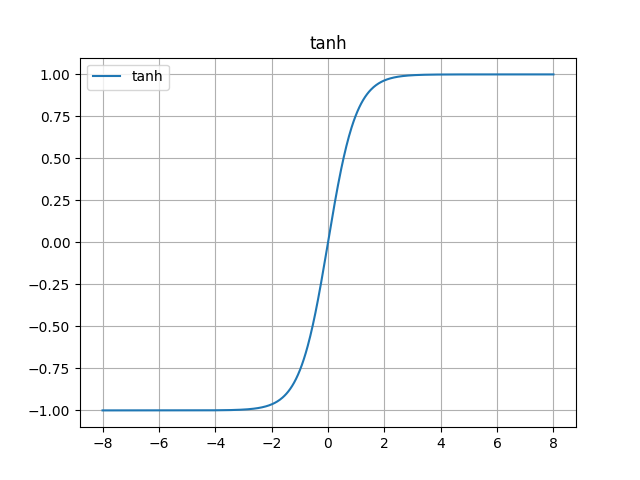
\includegraphics[width=0.45\textwidth]{tanh.png}
    \caption{Función tanh}
\end{figure}

La función Unidad Lineal Rectificada (ReLU, Rectified Linear Unit),

\begin{equation}
f(x) = \max(0, x)
\end{equation}

representada en la figura 2-6(a) tiene las siguientes características:
\begin{enumerate}
    \item Gradiente no saturado. Por el hecho de que \(x > 0\), el problema de la dispersión del gradiente en el proceso de propagación inversa se ve aliviado, y los parámetros en la primera capa de la red neuronal pueden actualizarse rápidamente. En \(x = 0\) no es derivable, por lo que es habitual asignar un valor arbitrario en este caso, por ejemplo 0, 0.5 o bien 1.0.
    \item Baja complejidad computacional. Dada su propia definición.
\end{enumerate}

No obstante, posee la desventaja de que la neurona ReLU puede morir cuando recibe un gradiente negativo alto durante la retropropagación que le permite aprender más porque su derivada es cero cuando su entrada es menor que cero, por lo que el gradiente será finalmente cero. Esto se puede evitar al inicializar cuidadosamente los pesos o utilizar ReLU con "fugas", similar a ReLU, pero donde su salida es lineal multiplicada por un valor pequeño (aproximadamente 0.001) cuando la entrada es negativa, esto es

\begin{equation}
f(x) = \max(0.01x, x)
\end{equation}

tal y como se muestra en la figura 2-6(b), conocida en ocasiones como ReLU con fugas (LReLU, Leaky ReLU).

\begin{figure}[h]
    \centering
    \includegraphics[width=0.45\textwidth]{relu.png}
    \includegraphics[width=0.45\textwidth]{lrelu.png}
    \caption{Funciones: (a) ReLU; (b) LReLU}
\end{figure}

En algunos tipos de redes como Mobile Net, que se estudiarán posteriormente, se define una variante de ReLU como sigue (es la función ReLU6), y cuya representación se muestra en la figura 2-7(a). A partir de ella se define hard-swish o h-swish (Hs) representada en la figura 2-7(b), aunque a veces en esta función se utiliza:

\begin{equation}
\text{ReLU6}(x) = \min(\max(x,0),6)
\end{equation}

\begin{equation}
\text{HS}(x) = x \cdot \frac{\text{ReLU6}(x + 3)}{6}
\end{equation}

\begin{figure}[h]
    \centering
    \includegraphics[width=0.45\textwidth]{relu6.png}
    \includegraphics[width=0.45\textwidth]{hswish.png}
    \caption{Funciones: (a) ReLU6; (b) Hard-Swish}
\end{figure}

La función Paramétrica ReLU (PReLU, Parametric ReLU, He y col., 2015b) se define según:

\begin{equation}
f(x, \alpha) = \begin{cases} 
x & \text{si } x > 0 \\ 
\alpha x & \text{si } x \leq 0 
\end{cases}
\end{equation}

De forma que si el parámetro \(\alpha = 0\) la función es exactamente ReLU; si \(\alpha > 0\) se trata de la función LReLU, es cuando el parámetro \(\alpha\) se incluye como un parámetro a aprender durante el proceso de entrenamiento, cuando la función toma su verdadero significado, de ahí su nombre.

Por otra parte, existe la Unidad lineal exponencial (ELU, Exponential Linear Unit) definida en Clevert y col. (2016) como sigue con \(\alpha > 0\):

\begin{equation}
f(x, \alpha) = \begin{cases} 
x & \text{si } x > 0 \\ 
\alpha (e^x - 1) & \text{si } x \leq 0 
\end{cases}
\end{equation}

El parámetro \(\alpha\) controla el valor para el cual se produce la saturación para valores de \(x\) negativos. En la figura 2-8 se muestran sendas funciones ELU con valores de \(\alpha = 0.1\) en (a) y 1.0 en (b), respectivamente.

\begin{figure}[h]
    \centering
    \includegraphics[width=0.45\textwidth]{elu_0.1.png}
    \includegraphics[width=0.45\textwidth]{elu_1.0.png}
    \caption{Funciones ELU: (a) con \(\alpha= 0.1\); (b) con \(\alpha= 1.0\)}
\end{figure}

La función SELU hace referencia a Unidad lineal exponencial escalada (Scaled Exponential Linear Unit), siendo una versión ligeramente modificada de ELU por Klambauer y col. (2017) y definida como sigue:

\begin{equation}
f(x, \alpha) = \begin{cases} 
\lambda x & \text{si } x > 0 \\ 
\lambda \alpha (e^x - 1) & \text{si } x \leq 0 
\end{cases}
\end{equation}

En la figura 2-9 se muestra la representación gráfica de la función SELU con valores \(\lambda = 1.0\) y \(\alpha = 2.0\).

\begin{figure}[h]
    \centering
    \includegraphics[width=0.45\textwidth]{selu.png}
    \caption{Función SELU}
\end{figure}

Las funciones ReLU tienen la ventaja de acelerar el entrenamiento, ya que el cálculo del gradiente es simple (0 o 1 dependiendo del signo de la entrada), y no existe una constante en la parte positiva del dominio.























\section{Introducción}
En este capítulo se inicia la presentación, junto con las características más relevantes de las redes neuronales profundas, que, desde sus primeros desarrollos a mediados del siglo XX, han recibido diferentes nombres entre los que destacan: redes neuronales, computadores neuronales, sistemas distribuidos paralelos, modelos conexionistas, entre otros.

Se inicia el capítulo con los fundamentos de este tipo de redes, para abordar a continuación el modelo del perceptrón, como unidad básica, y posteriormente la red de retropropagación. Se finaliza con una pincelada de los modelos conocidos como redes de creencia o bayesianas. En todos los casos con la vista puesta en el concepto de profundidad dentro del aprendizaje profundo.

\section{Fundamentos Generales}
El interés por las redes neuronales data de los años 40, a partir del trabajo de McCulloch y Pitts (1943), donde se proponen modelos de neuronas en la forma de dispositivos binarios basados en un umbral y algoritmos estocásticos que implicaban cambios binarios 0-1 y 1-0 en los estados de las neuronas como la base para el desarrollo de sistemas neuronales. El trabajo posterior de Hebb (1949) estaba basado en modelos matemáticos que intentaban capturar el concepto de aprendizaje por refuerzo o asociación. Durante la primera mitad de los años 50 y principios de los 60, las denominadas máquinas de aprendizaje propuestas por Rosenblatt (1962) supusieron una revolución entre los investigadores en la teoría de reconocimiento de patrones. La razón del gran interés de dichas máquinas llamadas perceptrones fue el desarrollo de las correspondientes demostraciones matemáticas llegando a la conclusión de que los perceptrones, cuando son entrenados con conjuntos de entrenamientos linealmente separables, convergen a una solución en un número finito de iteraciones. La solución tomó la forma de coeficientes de hiperplanos capaces de separar correctamente las clases representadas por patrones del conjunto de entrenamiento.

Desafortunadamente, las expectativas que siguieron a este descubrimiento perdieron fuerza porque el modelo anterior era inapropiado para muchas tareas de reconocimiento de patrones. Intentos posteriores para extender la potencia del perceptrón considerando múltiples capas de perceptrones fracasaron también. Un estado del arte sobre las máquinas de aprendizaje a mitad de los años 60 fue recopilado por Nilsson (1965). Unos pocos años más tarde, Minsky y Papert (1969) presentaron un estudio desalentador sobre las limitaciones de las máquinas de aprendizaje basadas en el perceptrón. Esta idea negativa se mantuvo hasta mitad de la década de los 80, llegándose incluso a rechazar el uso del perceptrón en algunos trabajos como el presentado por Simon (1986).

Los nuevos algoritmos de aprendizaje para perceptrones multicapa presentados por Rumelhart et al. (1986), conocidos como regla delta generalizada para aprendizaje por retropropagación, modificaron el interés por las redes neuronales. En los años sucesivos, nuevos algoritmos fueron presentados por diferentes autores. Aunque no se ha probado la convergencia de dichos algoritmos hacia una solución óptima, han sido aplicados con éxito a muchos problemas de interés práctico, lo que les otorgó una cierta validez en los años 90. A continuación, estas redes cayeron en popularidad en favor de otras técnicas diferentes. Los motivos fueron múltiples. Por ejemplo, no había un lenguaje estándar de facto para modelar redes neuronales. Tampoco se observaban mejoras significativas cuando se añadían muchas capas a la red, resultando a veces contraproducente. Además, el entrenamiento era computacionalmente costoso con los ordenadores disponibles en la época de referencia. Y en muchas condiciones no había suficientes datos para evitar el sobreajuste del modelo.

Para entender correctamente los fundamentos de las redes neuronales profundas conviene empezar estudiando el modelo más básico. Este consiste en especificar un conjunto de funciones indicador \(A(x,w)\) que toman los valores \{0,1\}, considerando que son los parámetros que definen cada posible elemento que hay que clasificar. Además, se considera que se dispone de \(n\) muestras \((x_i,y_i)\) de entrenamiento (con \(i=1,...,n\)) de las que se conoce su clase \(y_i\). A continuación se minimiza el riesgo empírico de la función indicador sobre todo elemento del conjunto de entrenamiento. Para ello se suele minimizar el error de clasificación incorrecta \(R_o(w) = \sum_i [f(x_i,w) - y_i]^2\).

Para entender mejor el proceso, considérese primero el siguiente caso especial de funciones indicador, donde \(h()\) es una función que indica si el elemento pertenece a la clase (toma el valor 1) o no (toma el valor 0) en base a la combinación lineal, sopesada por los valores de los pesos del modelo \(w\), de los \(q\) parámetros de entrada en \(x\).
\[
f(x,w) = h \left( \sum_{j=1}^q w_j x_j \right)
\]
En este caso, si se supone que el conjunto de datos de entrenamiento es linealmente separable, existe un simple procedimiento de optimización para encontrar \(f(x,w^*)\), que es conocido como el algoritmo del perceptrón. Cuando los datos son no separables este algoritmo no proporciona una solución óptima, motivo por el que se han desarrollado otros procedimientos. Uno de los métodos considerados es el entrenamiento conocido como Widrow-Hoff o regla delta de mínimos cuadrados, que minimiza una función del tipo dado en la ecuación anterior. Una alternativa diferente consiste en utilizar un perceptrón multicapa (MLP, Multi-Layer Perceptron), que es capaz de manejar adecuadamente tanto las clases separables como las no separables y que utiliza el riesgo empírico funcional dado por:
\[
R_{emp}(w,v) = \sum_{i=1}^n \left( f(x_i, w, v) - y_i \right)^2
\]
que debe ser minimizado con respecto a los parámetros o pesos \(w\) y \(v=[v_1, v_2, ..., v_m]\). En el caso del perceptrón multicapa, la función \(f(x,w,v)\) se parametriza como:
\[
f(x,w,v) = h \left( g(x, w, v) \right)
\]
donde \(g(x,w,v) = \sum_{j=1}^m v_j h \left( \sum_{i=1}^q w_{ji} x_i \right)\). 

\section{El Perceptrón}
El modelo más básico que se puede utilizar en los modelos de redes neuronales recibe el nombre de perceptrón. Debido a su expresión matemática, introducida brevemente en la sección anterior, es capaz de aprender el modelo (obtener los pesos en \(w\)) que permite distinguir los elementos de dos clases linealmente separables. En esta sección se detallan los elementos y formas de representar este modelo, y se explican diferentes métodos de entrenamiento para ajustar los valores de sus parámetros.

\subsection{Arquitectura del Perceptrón}
En su forma más básica, el perceptrón aprende una función discriminante lineal \(f_d(x)\) que se corresponde con la función \(f(x, w^*)\) introducida en la sección anterior. Esta función establece una dicotomía entre dos conjuntos de entrenamiento linealmente separables. Dados dos conjuntos de puntos, se dice que son linealmente separables si existe un hiperplano en el espacio patrón que separa ambos conjuntos de datos. En el caso de un espacio de dos dimensiones, el hiperplano se puede representar gráficamente y a efectos pedagógicos como una recta, tal y como se muestra en la Figura 3-1.

\begin{figure}[h]
    \centering
    \includegraphics[width=0.5\textwidth]{figura_3_1.png}
    \caption{Hiperplano de separación para el caso bidimensional}
    \label{fig:figura_3_1}
\end{figure}

La Figura 3-2(a) muestra el esquema del modelo del perceptrón para dos clases. La respuesta de este dispositivo está basada en dos etapas. En la primera, se calcula la suma promediada de sus entradas mediante una función de decisión lineal con respecto a las componentes de los vectores patrón:
\[
f_d(x) = \sum_{i=1}^n w_i x_i + w_{n+1}
\]
Los coeficientes \(w_i\), \(i= 1, 2, ..., n, n+1\), llamados pesos, modifican las entradas antes de que sean sumadas y suministradas al elemento de umbral. Una de las entradas es el sesgo (bias) externo \(w_{n+1}\). En este sentido, los pesos son similares a las sinapsis en el sistema neuronal humano.

En la segunda, se transforma la salida de la primera etapa mediante una función de activación (también conocida como función de transferencia). En su forma más simple, la función de activación es una función escalón (Figura 3-2(b)). Sin embargo, en otras arquitecturas de red también puede ser una función sigmoide o sigmoide binaria.

\begin{figure}[h]
    \centering
    \begin{subfigure}[b]{0.45\textwidth}
        \includegraphics[width=\textwidth]{figura_3_2a.png}
        \caption{}
        \label{fig:figura_3_2a}
    \end{subfigure}
    \begin{subfigure}[b]{0.45\textwidth}
        \includegraphics[width=\textwidth]{figura_3_2b.png}
        \caption{}
        \label{fig:figura_3_2b}
    \end{subfigure}
    \caption{Esquema del modelo del perceptrón para dos clases}
    \label{fig:figura_3_2}
\end{figure}

A continuación, se presenta un conjunto de ejemplos de patrones de entrada con el objetivo de encontrar el hiperplano que permite separar dos clases de forma adecuada. El conjunto de patrones de entrada es denotado como \(x_1, x_2, ..., x_n\), y cada patrón de entrada tiene una dimensión de \(m\). La salida deseada es denotada como \(d_1, d_2, ..., d_n\), donde cada \(d_i\) pertenece a \{0,1\}.


\end{comment}



\begin{comment}

\textbf{MXNet} \citep{mxnet} es un marco de trabajo de aprendizaje profundo de código abierto fundado como una colaboración entre la Universidad Carnegie Mellon, la Universidad de Washington y Microsoft. Es una librería escalable que permite el entrenamiento de redes neuronales profundas utilizando diferentes lenguajes de programación, incluyendo C++, Python, MATLAB, JavaScript, R, Julia y Scala. MXNet incluye la interfaz de Gluon que permite a los desarrolladores con cualquier nivel de experiencia comenzar a usar el aprendizaje profundo en la nube, en dispositivos de borde \footnote{dispositivos más cercanos al usuario, como teléfonos móviles, sistemas ciberfísicos (CPS), dispositivos portátiles, IoT, \ldots.} y en aplicaciones para dispositivos móviles. MXNet admite además el paralelismo de datos en múltiples CPUs o GPUs, así como el paralelismo de modelos. Ofrece dos modos de entrenamiento diferentes: síncrono y asíncrono \footnote{síncrono: interactúan en el mismo momento en el que tiene lugar la comunicación; asíncrono: la interacción no es inmediata y puede tener lugar en momentos diferentes} y además proporciona operaciones primitivas de tolerancia a fallas a través de guardar y cargar: guardar almacena los parámetros del modelo en un archivo de punto de control y cargar restaura los parámetros del modelo desde un archivo de punto de control. MXNet admite tanto la programación declarativa como la programación imperativa.
\textbf{Theano} \citep{theano} es una biblioteca de Python de código abierto para cálculos a gran escala que ha sido desarrollado por investigadores y desarrolladores de la Universidad de Montreal. Es una biblioteca que facilita la construcción de modelos de aprendizaje profundo y se puede ejecutar en diferentes plataformas informáticas, incluyendo CPU y GPU. Los cálculos se expresan utilizando una sintaxis similar a la de Numpy y funciona creando una representación simbólica de las operaciones que se traducen a C++ y luego se compilan en moléculas Python. Theano admite tanto el paralelismo de datos como el paralelismo de modelos.
\textbf{Chainer} \citep{chainer} es un marco de aprendizaje profundo de código abierto implementado en Python. El desarrollo de Chainer está liderado por investigadores y desarrolladores de la Universidad de Tokio. Chainer proporciona APIs de diferenciación automática para construir y entrenar redes neuronales, con un enfoque de ``definir por ejecutar'', lo que permite construir el grafo computacional durante el entrenamiento y permite al usuario cambiarlo en cada iteración. Chainer es un marco flexible ya que proporciona una API imperativa en Python y NumPy. Se admiten tanto cálculos en CPU como en GPU.
\end{comment}









